\chapter{Παράγωγος Σύνθετων Συναρτήσεων}

\section{1η Περίπτωση: \ensuremath{z=f(x,y),  x=x(t),  y=y(t)}} 

\begin{thm}
  Αν η συνάρτηση $ f(x,y) $ είναι ορισμένη στο ανοιχτό σύνολο 
  $ A \subseteq \mathbb{R}^{2} $ και $ x = x(t) $, $ y=y(t) $, με 
  $ t \in [a,b] $ και η $f$ έχει συνεχείς μερικές 
  παραγώγους στο $A$ και οι $ x(t) $ και $ y(t) $ είναι παραγωγίσιμες στο 
  $ [a,b] $, τότε η παράγωγος της σύνθετης συνάρτησης $f$ ως προς $t$ δίνεται από 
  τον τύπο:

  \vspace{\baselineskip}

  \twocolumnsideslc{
    \begin{center}
      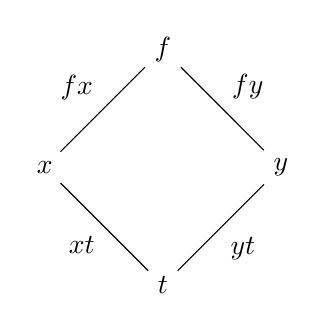
\begin{tikzpicture}
        \node (f) at (0,0) {$f$};  
        \node (x) at (-1.5,-1.5) {$x$};  
        \node (y) at (1.5,-1.5) {$y$};  
        \node (t) at (0,-3) {$t$};  
        \draw (f) edge node[midway,above left] {$\pdv{f}{x}$} (x) ;
        \draw (f) edge node[midway,above right] {$\pdv{f}{y}$} (y) ;
        \draw (x) edge node[midway,below left] {$\dv{x}{t}$} (t) ;
        \draw (y) edge node[midway,below right] {$\dv{y}{t}$} (t) ;
      \end{tikzpicture}
    \end{center}
  }{
    \begin{equation}\label{eq:deriv1}
      \dv{f}{t} = \pdv{f}{x} \dv{x}{t} + \pdv{f}{y} \dv{y}{t} 
    \end{equation}
    Ενώ η 2η παράγωγος από τον τύπο:
    \[
      \dv[2]{f}{t} =  \pdv[2]{f}{x} \left(\dv{x}{t}\right)^{2} + 
      2 \pdv[2]{f}{x}{y} \dv{x}{t} \dv{y}{t} + \pdv[2]{f}{y} 
      \left(\dv{y}{t}\right)^{2} + \pdv{f}{x} \dv[2]{x}{t} + \pdv{f}{y} \dv[2]{y}{t}
    \]
  }
\end{thm}

\section{2η Περίπτωση: \ensuremath{z=f(x,y),  x=x(u,v),  y=y(u,v)}} 

\begin{thm}
  Αν η συνάρτηση $ f(x,y) $ είναι ορισμένη στο ανοιχτό σύνολο 
  $ A \subseteq \mathbb{R}^{2} $ και $ x = x(u,v) $, $ y=y(u,v) $, με 
  και η $f$ έχει συνεχείς μερικές παραγώγους στο $A$ και οι $ x $ και $ y $, έχουν 
  συνεχείς μερικές παραγώγους στο $ E \subseteq \mathbb{R}^{2} $,
  τότε οι μερικές παράγωγοι της $f$, υπάρχουν και δίνονται από τους τύπους:
\end{thm}

\twocolumnsideslc{ 
  \begin{center}
    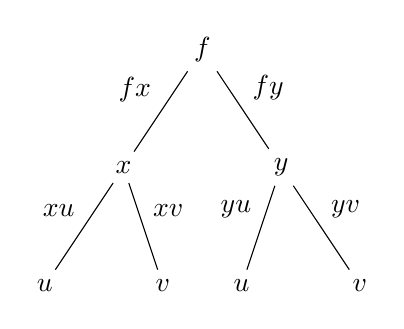
\begin{tikzpicture}
      \node (f) at (0,0) {$f$};  
      \node (x) at (-1,-1.5) {$x$};  
      \node (y) at (1,-1.5) {$y$};  
      \node (ux) at (-2,-3) {$u$};  
      \node (vx) at (-0.5,-3) {$v$};  
      \node (uy) at (0.5,-3) {$u$};  
      \node (vy) at (2,-3) {$v$};  
      \draw (f) edge node[midway,above left] {$ \pdv{f}{x}$} (x) ;
      \draw (f) edge node[midway,above right] {$ \pdv{f}{y}$} (y) ;
      \draw (x) edge node[midway,above left] {$ \pdv{x}{u}$} (ux) ;
      \draw (x) edge node[midway,above right] {$ \pdv{x}{v}$} (vx) ;
      \draw (y) edge node[midway,above left] {$ \pdv{y}{u}$} (uy) ;
      \draw (y) edge node[midway,above right] {$ \pdv{y}{v}$} (vy) ;
    \end{tikzpicture}  
  \end{center}
}{
  \begin{equation}
    \label{eq:deriv2}
    \pdv{f}{u} = \pdv{f}{x} \pdv{x}{u} + \pdv{f}{y} \pdv{y}{u} 
    \quad \text{και} \quad
    \pdv{f}{v} = \pdv{f}{x} \pdv{x}{v} + \pdv{f}{y} \pdv{y}{v} 
  \end{equation}
  Ενώ οι μερικές παράγωγοι 2ης τάξης, δίνονται από τους τύπους:
  \[
    \pdv[2]{f}{u} =  \pdv[2]{f}{x} \left(\pdv{x}{u}\right)^{2} + 
    2 \pdv[2]{f}{x}{y} \pdv{x}{u} \pdv{y}{u} + \pdv[2]{f}{y} 
    \left(\pdv{y}{u}\right)^{2} + \pdv{f}{x} \pdv[2]{x}{u} + \pdv{f}{y} 
    \pdv[2]{y}{u}
  \]
  \[
    \pdv[2]{f}{v} =  \pdv[2]{f}{x} \left(\pdv{x}{v}\right)^{2} + 
    2 \pdv[2]{f}{x}{y} \pdv{x}{u} \pdv{y}{v} + \pdv[2]{f}{y} 
    \left(\pdv{y}{v}\right)^{2} + \pdv{f}{x} \pdv[2]{x}{v} + \pdv{f}{y} 
    \pdv[2]{y}{v}
  \]
  \[
    \pdv[2]{f}{v}{u} = \pdv[2]{f}{x} \pdv{x}{u} \pdv{x}{v} + \pdv[2]{f}{x}{y}
    \left(\pdv{x}{u} \pdv{y}{v}+ \pdv{x}{v} \pdv{y}{u} \right) + \pdv[2]{f}{y} 
    \pdv{y} {u} \pdv{y}{v} + \pdv{f}{x} \pdv[2]{x}{u}{v} + \pdv{f}{y} 
    \pdv[2]{y}{u}{v} 
  \]
}


\enlargethispage{\baselineskip}

\begin{rem}
  Οι τύποι~\eqref{eq:deriv1} και~\eqref{eq:deriv2} προέκυψαν αθροίζοντας κάθε φορά, 
  τα μονοπάτια που ξεκινούν από τη μεταβλητή $f$ και καταλήγουν στη μεταβλητή ως 
  προς την οποία παραγωγίζουμε, όπου κάθε μονοπάτι αποτελείται από το γινόμενο των 
  παραγώγων που συναντούμε "διασχίζοντάς" το.
\end{rem}


\section{Αποδείξεις των τύπων των μερικών Παραγώγων 2ης τάξης}

\subsection{Απόδειξη με το συμβολισμό του Leibnitz}

Αποδεικνύουμε τον τύπο για την $ \pdv[2]{f}{u} $ και ομοίως προκύπτουν και οι τύποι 
για τις $ \pdv[2]{f}{v}  $ και $ \pdv[2]{f}{u}{v} $.

\vspace{\baselineskip}

\twocolumnsideslc
{
  \begin{center}
    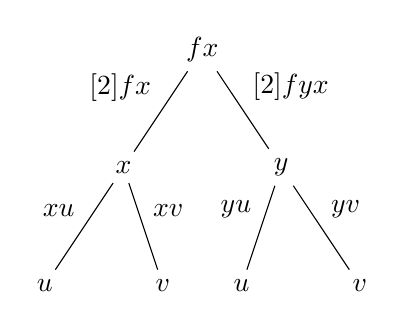
\begin{tikzpicture}
      \node (f) at (0,0) {$ \pdv{f}{x} $};  
      \node (x) at (-1,-1.5) {$x$};  
      \node (y) at (1,-1.5) {$y$};  
      \node (ux) at (-2,-3) {$u$};  
      \node (vx) at (-0.5,-3) {$v$};  
      \node (uy) at (0.5,-3) {$u$};  
      \node (vy) at (2,-3) {$v$};  
      \draw (f) edge node[midway,above left] {$ \pdv[2]{f}{x}$} (x) ;
      \draw (f) edge node[midway,above right] {$ \pdv[2]{f}{y}{x}$} (y) ;
      \draw (x) edge node[midway,above left] {$ \pdv{x}{u}$} (ux) ;
      \draw (x) edge node[midway,above right] {$ \pdv{x}{v}$} (vx) ;
      \draw (y) edge node[midway,above left] {$ \pdv{y}{u}$} (uy) ;
      \draw (y) edge node[midway,above right] {$ \pdv{y}{v}$} (vy) ;
    \end{tikzpicture}  
  \end{center}

  \begin{center}
    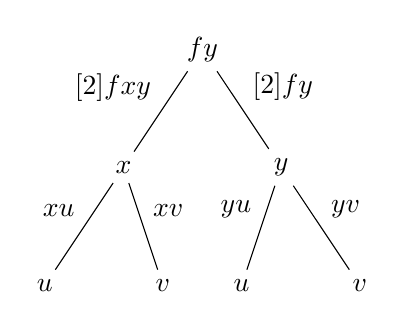
\begin{tikzpicture}
      \node (f) at (0,0) {$ \pdv{f}{y} $};  
      \node (x) at (-1,-1.5) {$x$};  
      \node (y) at (1,-1.5) {$y$};  
      \node (ux) at (-2,-3) {$u$};  
      \node (vx) at (-0.5,-3) {$v$};  
      \node (uy) at (0.5,-3) {$u$};  
      \node (vy) at (2,-3) {$v$};  
      \draw (f) edge node[midway,above left] {$ \pdv[2]{f}{x}{y}$} (x) ;
      \draw (f) edge node[midway,above right] {$ \pdv[2]{f}{y}$} (y) ;
      \draw (x) edge node[midway,above left] {$ \pdv{x}{u}$} (ux) ;
      \draw (x) edge node[midway,above right] {$ \pdv{x}{v}$} (vx) ;
      \draw (y) edge node[midway,above left] {$ \pdv{y}{u}$} (uy) ;
      \draw (y) edge node[midway,above right] {$ \pdv{y}{v}$} (vy) ;
    \end{tikzpicture}  
  \end{center}
}{
  \begin{proof}
    \[
      \begin{aligned}
        \pdv[2]{f}{u} 
  &= \pdv{}{u}\left(\pdv{f}{u}\right) = \pdv{}{u} 
  \left( \pdv{f}{x} \pdv{x}{u} + \pdv{f}{y} \pdv{y}{u}\right) = 
  \pdv{}{u} \left(\pdv{f}{x} \pdv{x}{u}\right) + \pdv{}{u} 
  \left(\pdv{f}{y} \pdv{y}{u}\right) \\
  &= \pdv{}{u} \left( \pdv{f}{x}\right) \pdv{x}{u} + \pdv{f}{x} \pdv{}{u} \left(
  \pdv{x}{u} \right) + \pdv{}{u} \left(\pdv{f}{y} \right) \pdv{y}{u} + \pdv{f}{y} 
  \pdv{}{u} \left(\pdv{y}{u}\right) \\
  &=\left[ \pdv[2]{f}{x} \pdv{x}{u} + \pdv[2]{f}{x}{y} \pdv{y}{u} \right] \pdv{x}{u} +
  \pdv{f}{x} \pdv[2]{x}{u} + 
  \left[ \pdv[2]{f}{y}{x} \pdv{x}{u} + \pdv[2]{f}{y} \pdv{y}{u} \right] \pdv{y}{u} +
  \pdv{f}{y} \pdv[2]{y}{u} \\
  &= \pdv[2]{f}{x} \left(\pdv{x}{u}\right)^{2} + \pdv[2]{f}{x}{y} \pdv{y}{u}
  \pdv{x}{u} + \pdv{f}{x} \pdv[2]{x}{u} + \pdv[2]{f}{y}{x} \pdv{x}{u} \pdv{y}{u} + 
  \pdv[2]{f}{y} \left(\pdv{y}{u}\right)^{2} +
  \pdv{f}{y} \pdv[2]{y}{u} \\
  &= \pdv[2]{f}{x} \left(\pdv{x}{u}\right)^{2} + 2\pdv[2]{f}{x}{y} \pdv{x}{u}
  \pdv{y}{u} + \pdv[2]{f}{y} \left(\pdv{y}{u}\right)^{2} + \pdv{f}{x} \pdv[2]{x}{u} +
  \pdv{f}{y} \pdv[2]{y}{u} \\
      \end{aligned}
    \]
  \end{proof}
}


\subsection{Απόδειξη με το συμβολισμό των δεικτών}

Αποδεικνύουμε τον τύπο για την $ f_{uu} $ και ομοίως προκύπτουν και οι τύποι για τις  
$ f_{vv} $ και $ f_{uv} $.

\vspace{\baselineskip}

\twocolumnsideslc{
\begin{center}
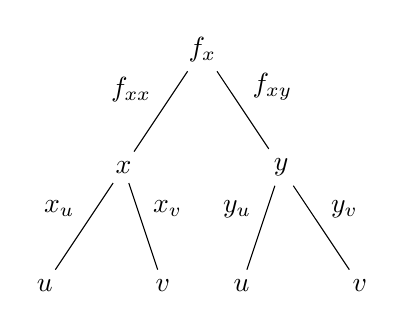
\begin{tikzpicture}
  \node (f) at (0,0) {$f_{x}$};  
  \node (x) at (-1,-1.5) {$x$};  
  \node (y) at (1,-1.5) {$y$};  
  \node (ux) at (-2,-3) {$u$};  
  \node (vx) at (-0.5,-3) {$v$};  
  \node (uy) at (0.5,-3) {$u$};  
  \node (vy) at (2,-3) {$v$};  
  \draw (f) edge node[midway,above left] {$f_{xx}$} (x) ;
  \draw (f) edge node[midway,above right] {$f_{xy}$} (y) ;
  \draw (x) edge node[midway,above left] {$x_{u}$} (ux) ;
  \draw (x) edge node[midway,above right] {$x_{v}$} (vx) ;
  \draw (y) edge node[midway,above left] {$y_{u}$} (uy) ;
  \draw (y) edge node[midway,above right] {$y_{v}$} (vy) ;
\end{tikzpicture}
\end{center}

\begin{center}
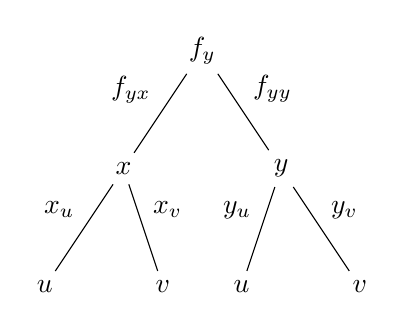
\begin{tikzpicture}
  \node (f) at (0,0) {$f_{y}$};  
  \node (x) at (-1,-1.5) {$x$};  
  \node (y) at (1,-1.5) {$y$};  
  \node (ux) at (-2,-3) {$u$};  
  \node (vx) at (-0.5,-3) {$v$};  
  \node (uy) at (0.5,-3) {$u$};  
  \node (vy) at (2,-3) {$v$};  
  \draw (f) edge node[midway,above left] {$f_{yx}$} (x) ;
  \draw (f) edge node[midway,above right] {$f_{yy}$} (y) ;
  \draw (x) edge node[midway,above left] {$x_{u}$} (ux) ;
  \draw (x) edge node[midway,above right] {$x_{v}$} (vx) ;
  \draw (y) edge node[midway,above left] {$y_{u}$} (uy) ;
  \draw (y) edge node[midway,above right] {$y_{v}$} (vy) ;
\end{tikzpicture}
\end{center}
}{
  \begin{proof}
    \[
      \begin{aligned}
        f_{uu} &= (f_{u})_{u} = (f_{x}x_{u}+f_{y}y_{u})_{u} \\
               &=(f_{x}x_{u})_{u}+ (f_{y}y_{u})_{u} \\
               &=(f_{x})_{u}x_{u} + f_{x}(x_{u})_{u} + (f_{y})_{u}y_{u}+ 
               f_{y}(y_{u})_{u} \\
               &= (f_{xx}x_{u}+f_{xy}{y_{u}})x_{u} + f_{x} x_{uu} + 
               (f_{yx}x_{u}+f_{yy}y_{u})y_{u} + f_{y}y_{uu} \\
               &= f_{xx}(x_{u})^{2} + f_{xy}y_{u}x_{u}+ f_{x}x_{uu} + 
               f_{yx}x_{u}y_{u}+f_{yy}(y_{u})^{2}+ f_{y}y_{uu} \\
               &= f_{xx}(x_{u})^{2}+ 2f_{xy}x_{u}y_{u} + f_{yy}(y_{u})^{2} + 
               f_{x}x_{uu} + f_{y}y_{uu}
      \end{aligned}
    \] 
  \end{proof}
}

\begin{rem}
  Συγκεντρωτικά οι τύποι για τις παραγώγους 2ης τάξης της συνάρτησης 
  \[
    f_{uu}= f_{xx}(x_{u})^{2}+ 2f_{xy}x_{u}y_{u} + f_{yy}(y_{u})^{2} + f_{x}x_{uu} + 
    f_{y}y_{uu} 
  \] 
  \[
    f_{vv}= f_{xx}(x_{v})^{2}+ 2f_{xy}x_{v}y_{v} + f_{yy}(y_{v})^{2} + f_{x}x_{vv} + 
    f_{y}y_{vv} 
  \]
  \[
    f_{uv}= f_{xx}x_{u}x_{v}+ f_{xy}(x_{u}y_{v} + x_{v}y_{u}) + 
    f_{yy}y_{u}y_{v} + f_{x}x_{uv} + f_{y}y_{v} 
    f_{y}y_{vv} 
  \]
\end{rem}



